\documentclass[a4paper]{article}
\usepackage[utf8]{inputenc}
\usepackage{polski}
\usepackage{graphicx}
\title{Pół-autonomiczny pojazd czterokołowy}
\author{Jędrzej Maliniak \and Piotr Hebel \and Filip Malinowski \and Piotr Dulewicz \and Piotr Jabłoński \and Andrzej Szmyt}
\date{7 marca 2016}

\begin{document}

\maketitle

\section{Problem projektu}
    Przedmiotem tego projektu jest pół-autonomiczny pojazd czterokołowy wyposażony w kamerę wykorzystywaną do transmisji obrazu do stacji operatorskiej i dwustopniowy system detekcji kolizji, na który składają się sensory ultradźwiękowe, jako pierwszy stopień systemu detekcji kolizji, mierzące odległość od obiektów otoczenia wykorzystywane również do orientacji oraz czujniki stykowe (w tej roli czujniki krańcowe z dźwignią) jako drugi - ostateczny - stopień  detekcji kolizji. W przypadku otrzymania sygnału z czujników krańcowych - świadczącego o niebezpiecznie bliskiej odległości od przeszkody - pojazd zatrzyma się, jest to decyzja ostateczna i niezaprzeczalna dająca możliwość osobie sterującej otrzymanie obrazu bieżącej pozycji (już po np. opóźnieniach czy innego typu problemach z przysyłaniem danych). W przyszłości zespół ma nadzieję na rozwój projektu wzbogacając go o m.in. możliwość mapowania otoczenia, umożliwić interfejs do komunikacji z montowanym działem laserowym czy prostym manipulatorem/ramieniem/chwytakiem umożliwiającym zbieranie próbek terenu czy wykonywanie prostych operacji na napotkanych obiektach.
    
    Spodziewany wynik prac to wyżej opisany zdalnie sterowany pojazd bezzałogowy który będzie spełniał kryteria ewaluacji opisane w dokumencie pt. ,,Założenia projektowe, specyfikacja funkcjonalna, kryteria ewaluacji".

    Wyniki będą umieszczane w archiwum wraz z oprogramowaniem, dokumentacją algorytmów, oprogramowania, układu mechanicznego i elektronicznego, przykładami działania oraz dokumentacja multimedialną w postaci zdjęć lub/i nagrań przedstawiających wczesne fazy rozwoju oraz testy.
\section{Plan pracy}
    Na następnej stronie znajduje się wykres Gantta prezentujący podział oraz rozplanowanie zadań w czasie. Dekompozycja układów mechanicznego, elektronicznego oraz oprogramowania wraz ze szczegółowymi opisami i osobami odpowiedzialnymi za poszczególne komponenty znajdują się w dokumencie pt. ,,Założenia projektowe, specyfikacja funkcjonalna, kryterium ewaluacji".    
        \begin{figure}
            \centering
            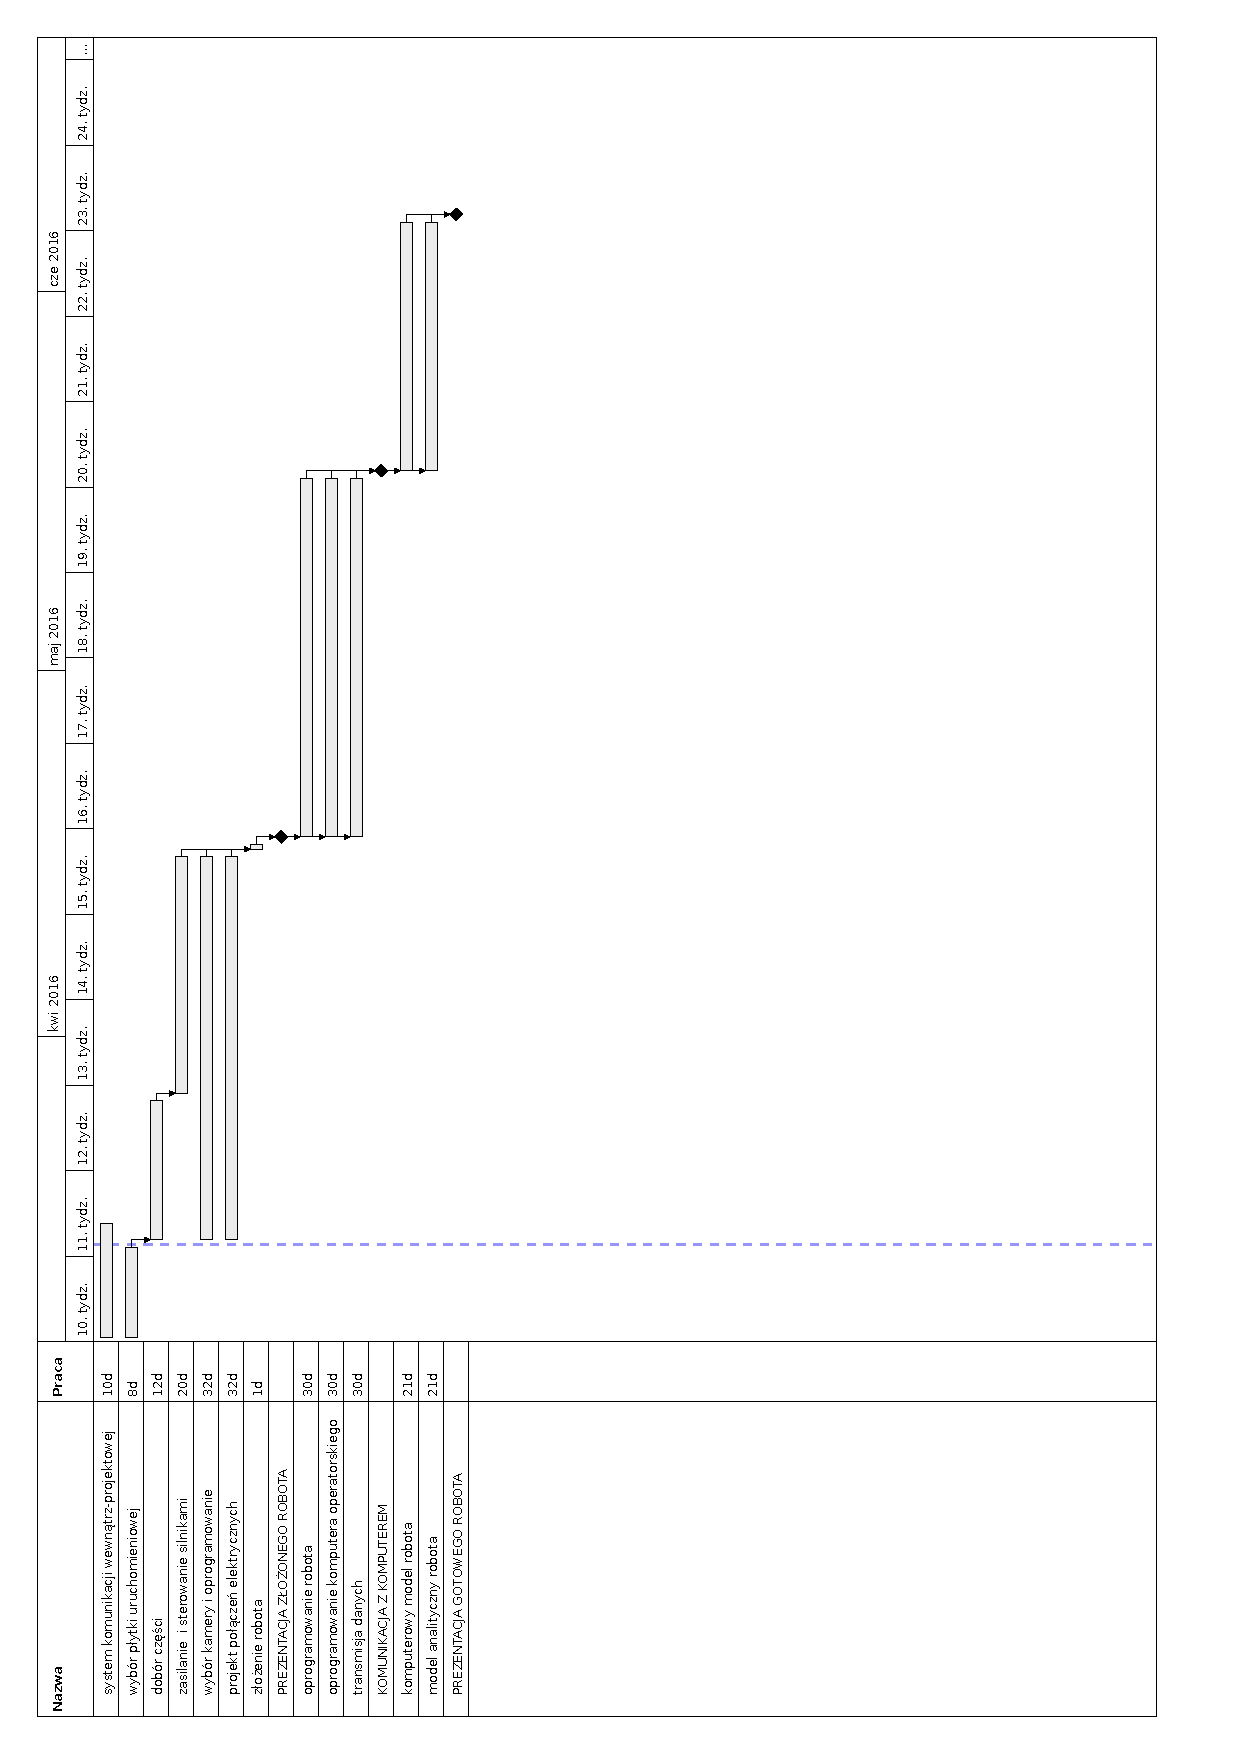
\includegraphics[scale=0.7]{autko}
            \label{fig:my_label}
        \end{figure}
\newpage
\section{Doręczenie}
    Raporty i postępy będą prezentowane w terminach zaznaczonych w diagramie Gantta jako kamienie milowe:
    \begin{itemize}
        \item Prezentacja złożonego robota - 17 kwietnia
        \item Komunikacja z komputerem - 17 maja
        \item Prezentacja gotowego robota - 7 czerwca
    \end{itemize}
\section{Budżet}
   \begin{center}
    \begin{tabular}{|c|c|c|}
        \hline
         Nazwa  & ilość & Cena Brutto \\
        \hline
         Koło + silnik 65x26mm 5V z przekładnią 48:1 & 4 & 87,60 zł \\
        \hline
        Czujniki ultradźwiękowe HC-SR04 2-200cm & 3 & 29,70 zł\\
        \hline
        L293D - dwukanałowy sterownik silników 36V/0.6A & 2 & 13,90 zł\\
        \hline
        Stabilizator 5V L7805CV - THT TO220 & 2 & 1,60 zł\\
        \hline
        Kondensator ceramiczny 330pF/50V THT - 10 szt. & 1 & 0,99 zł\\
        \hline
        Kondensator ceramiczny 150pF/50V THT - 10 szt. & 1 & 0,99 zł\\
        \hline
        Camera HD B - kamera ze zmienną ogniskową dla Raspberry Pi & 1 & 84,00 zł\\
        \hline
        Płytka uniwersalna PDU11 - THT & 1 & 8,40 zł\\
        \hline
        Wyłącznik czujnik krańcowy mini z dźwignią zakrzywioną - WK330 & 8 & 9,60 zł\\
        \hline
        Koszty transportu & 1 & 12,90 zł\\
        \hline
        Cena łączna & & 249,68 zł\\
        \hline
    \end{tabular}
    \end{center}
\section{Zarządzanie projektem}
    \subsection{Standardy wykorzystywane podczas pracy nad projektem}
    \begin{itemize}
        \item \LaTeX - do tworzenia dokumentacji
        \item planner - do tworzenia diagramu Gantta
        \item git - zdecentralizowany system do kontroli wersji
        \item trac - do rozdzielania zadań do wykonania (współpracuje z gitem)
        \item doxygen - do dokumentowania kodu
        \item TopSolid - do tworzenia komputerowego modelu robota
    \end{itemize}
    Regularne spotkania będą odbywały się w uprzednio wybrany dzień weekendu. Konflikty będą poddawane demokratycznej debacie a w razie braku konsensusu koordynator ma rozstrzygający głos.
\section{Integracja}
    Jako, że nad kodem oraz dokumentacją pracuje wiele osób zdecydowano się na użycie zdecentralizowanego systemu kontroli wersji git. Za spójność dokumentów zawartych w repozytorium odpowiada lider zespołu - Jędrzej Maliniak - oraz Filip Malinowski. Osoby te są również odpowiedzialne za nadzór i integrację danych znajdujących się na dysku sieciowym zawierającym dokumentacje, materiały multimedialne, etc. 
\section{Zespół}
    \subsection{Jędrzej Maliniak}
    Koordynator projektu - przydzielanie i nadzór zadań wykonywanych przez członków grupy, zarządzanie projektem.
        \begin{itemize}
            \item Budowa robota
            \item Oprogramowanie robota
            \item Kwestia komunikacji bezprzewodowej
            \item Opracowanie algorytmów
            \item Kwestie programistyczne
        \end{itemize}
    \subsection{Piotr Dulewicz}
        \begin{itemize}
            \item Oprogramowanie robota
            \item Projekt komputerowy
        \end{itemize}
    \subsection{Piotr Hebel}
        \begin{itemize}
            \item Budowa robota
            \item Kwestia komunikacji bezprzewodowej
            \item Projekt komputerowy
        \end{itemize}
    \subsection{Filip Malinowski}
        \begin{itemize}
            \item Kinematyka robota
            \item Opracowanie algorytmów
            \item Kwestie programistyczne
            \item Projekt komputerowy
        \end{itemize}
    \subsection{Piotr Jabłoński}
        \begin{itemize}
            \item Budowa robota
            \item Kwestie programistyczne
            \item Projekt komputerowy
        \end{itemize}
    \subsection{Andrzej Szmyt}
        \begin{itemize}
            \item Budowa robota
            \item Kwestia komunikacji bezprzewodowej
            \item Projekt komputerowy
        \end{itemize}
        

\end{document}
